\chapter{Simulation}\label{ch:simulation}

To ensure the functionality and robustness of the implemented offloading pipeline, the experiments are first carried out in simulation. \Cref{sec:simulation:experiment_setup} describes the implementation of the simulation experiments in details. In \cref{sec:simulation:results_and_discussion}, the evaluated experiment results are presented and discussed. 

\section{Experiment Setup}\label{sec:simulation:experiment_setup}

This section describes the implementation of the simulation experiments. More specifically, this section describes how the \gls{amr}'s onboard system and the edge computer are simulated as well as the resource limitation and network. This section is built upon \cref{sec:general_setup:implementation}, which describes the general setup for experiments. As mentioned in \cref{sec:general_setup:implementation}, the \gls{amr}'s onboard system and the edge computer are virtualized by \gls{docker} containers. The \gls{docker} containers in use are built upon the \gls{linux} docker containers with the \gls{ros} and \gls{pytorch} dependencies installed. In \cref{fig:simulation_experiment_setup}, the distribution of different modules among the containers and the host machine is illustrated. 

% TODO: adapt this figure
\begin{figure}[htp]
    \centering
    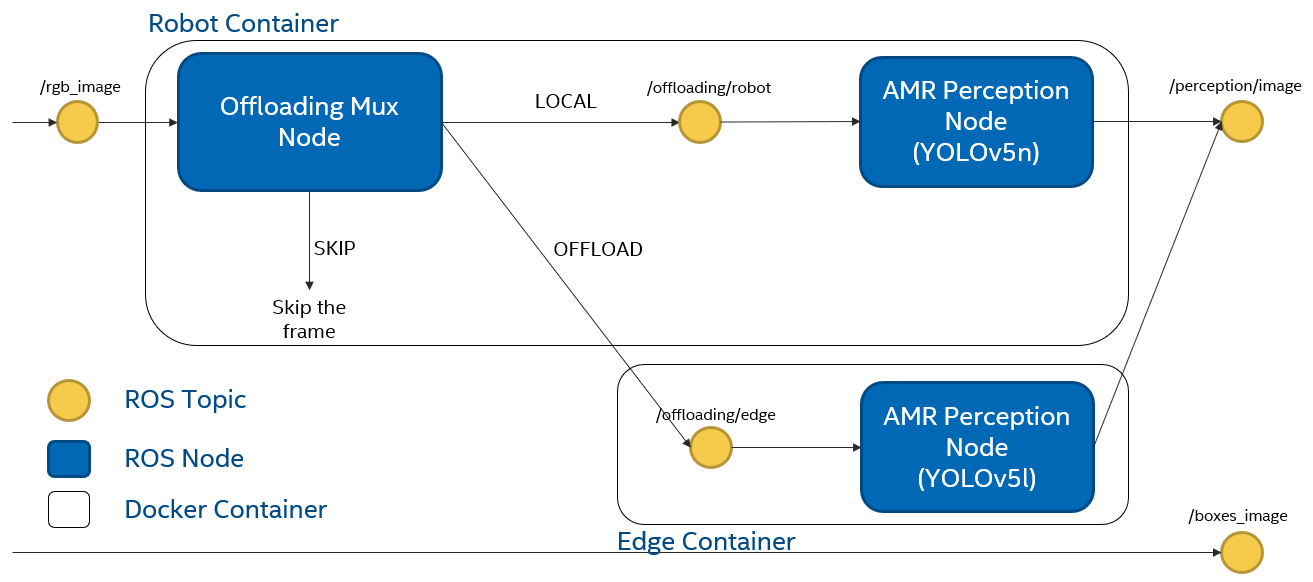
\includegraphics[width=0.8\linewidth]{figures/setup/general_setup.png}
    \caption{Simulation experiment setup}
    \label{fig:simulation_experiment_setup}
\end{figure}

\subsection{Resource Limitation Simulation}

The host machine is equipped with an Intel(R) Core(TM) i9-7900X \gls{cpu} and a Nvidia GeForce GTX 1060 6GB \gls{gpu}. The \gls{cpu} has a total of 20 cores. In order to simulate the \gls{amr}'s and the edge computer in realistic conditions, this thesis limits the computation resources of the \gls{docker} containers. The robot container is constrained to using only eight cores of the host machine, while the edge container is given ten cores. In addition, the edge computer has the access to the \gls{gpu} of the host machine and calculates the image inference on the \gls{gpu}. Moreover, the robot container is also constrained to using only 4 GB of memory, while the memory of the edge container is not constrained and the host machine has access to 32 GB of memory, including the 4 GB memory assigned to the robot container.

The limitations of CPU and memory usage are realized by tools provided by \gls{docker} itself. According to the \gls{docker} documentation, the runtime memory limitation is realized by Memory Resource Controller provided by the \gls{linux} kernel. Furthermore, the \gls{docker} container can enforce hard memory limitation and soft memory limitation at runtime. The former does not allow the container to use any amount more than specified, while the latter only kicks in when certain conditions are met. In this thesis, we use the hard memory limitation on the robot container to simulate the hardware constraints. For CPU usage, the limitation is realized by the CFS scheduler, which is the \gls{linux} kernel CPU scheduler for normal \gls{linux} processes. This indicates that the limitation on CPU usage is achieved by limiting the accessible CPU cycles of the \gls{docker} container. The GPU of the host machine is exposed to the \gls{docker} containers using the Nvidia Container Toolkits.

\subsection{Network Simulation}

In addition to resource limitation simulation, the network is also simulated to achieve realistic conditions for the robot and edge containers. The containers use the default \gls{docker} bridge network. Since the simulated scenario \gls{ros} bag is replayed in the robot container and the output data are also recorded in the robot container, the data flow between the robot container and the edge container only consists of offloaded images and detection processed by the edge container. To allow the data flow of 30 frames per second of images with resolution of 848 x 640 pixels, which is around 40 MB per second, the packet limit of in and out policies of the \gls{netem} is set to 20000. The in and out delays are set to 50 ms for both policies. To investigate the influence of the network bandwidth, the experiments are carried out under two bandwidth conditions: with 160 Mbit/s bandwidth constraint and no bandwidth constraints at all. The former aims to represent a limited network bandwidth that is unable to handle the data flow that is needed for a full offloaded execution, while the latter one represents a unlimited network bandwidth. 

For \gls{qos} settings, the offloading module uses "best effort" reliable policy to prevent the the publisher from being blocked by the bag network connection caused by the bandwidth constraints. As mentioned in \cref{sec:background:frameworks}, only \gls{fast_dds} allows a true asynchronous publishing mode. Therefore, Fast-DDS is used for \gls{ros} middle ware and the publishing mode is set to asynchronous for the experiments. The offloading module uses the "keep last" queuing settings and the queue size is set to 5. Furthermore, the \gls{ros} bag replay of the simulated scenario and the state monitors also use "best effort" reliable policy settings to simulate a camera sensor. 



\section{Results and Discussion}\label{sec:simulation:results_and_discussion}

% TODO: add tables for results
In this section, the results of the metrics with different offloading strategies are presented and analyzed. The results of the task performance metrics are shown from \cref{fig:simulation:processed_frame_percentage} to \cref{fig:simulation:map}. The results of the \gls{amr}'s onboard resources are shown from (refer to a figure here) to (refer to a figure here). 

\subsection{Analysis of task performance}

% The results in \cref{fig:simulation:map} show that offloading 80 percent of the images gives the best results in object detection task. It shows poor results when only computing the images locally (RobotOnly). This shows that the robot container cannot process the object detection due to the computational constraints. This can be also observed in

\begin{figure}[htp]
    \centering
    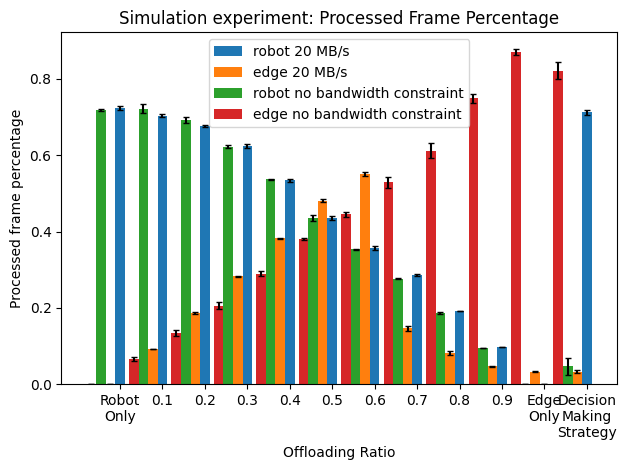
\includegraphics[width=\linewidth]{figures/experiment/simulation/processed_frame_percentage.png}
    \caption{Simulation experiment: processed frame percentage}
    \label{fig:simulation:processed_frame_percentage}
\end{figure}

\begin{figure}[htp]
    \centering
    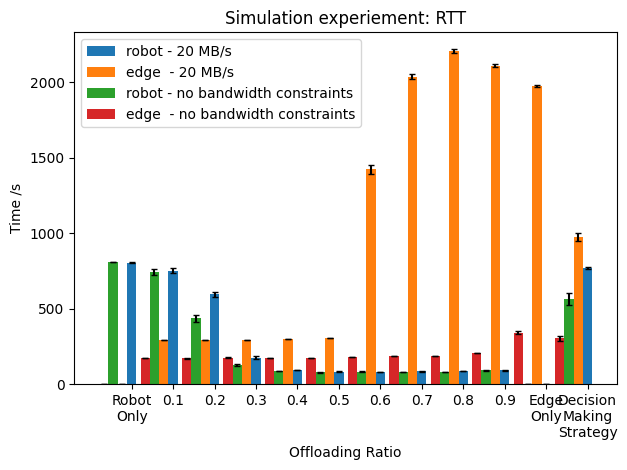
\includegraphics[width=\linewidth]{figures/experiment/simulation/rtt.png}
    \caption{Simulation experiment: \Gls{rtt}}
    \label{fig:simulation:rtt}
\end{figure}

\begin{figure}[htp]
    \centering
    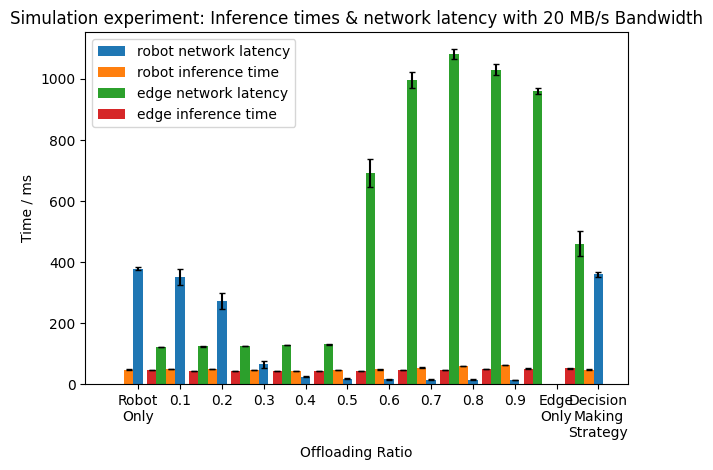
\includegraphics[width=\linewidth]{figures/experiment/simulation/execution_time_160.png}
    \caption{Simulation experiment: Execution time with 160 Mbit/s bandwidth}
    \label{fig:simulation:execution_time_160}
\end{figure}

\begin{figure}[htp]
    \centering
    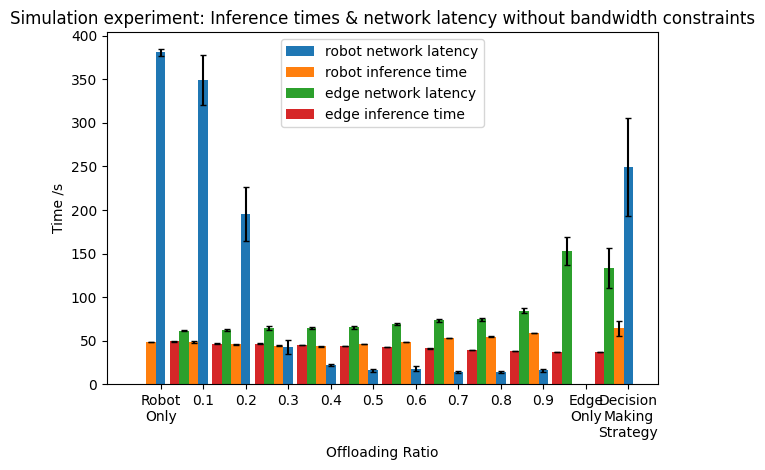
\includegraphics[width=\linewidth]{figures/experiment/simulation/execution_time_320.png}
    \caption{Simulation experiment: Execution time with 320 Mbit/s bandwidth}
    \label{fig:simulation:execution_time_320}
\end{figure}

\begin{figure}[htp]
    \centering
    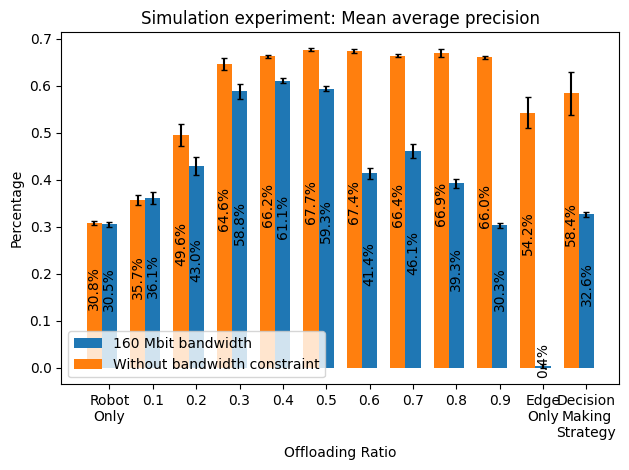
\includegraphics[width=\linewidth]{figures/experiment/simulation/map.png}
    \caption{Simulation experiment: \gls{map} with different bandwidths}
    \label{fig:simulation:map}
\end{figure}


\subsection{Analysis of onboard resources}

% \begin{figure}
%     \centering
%     \begin{subfigure}[htp]{0.45\linewidth}
%         \centering
%         \includegraphics[width=\linewidth]{figures/experiment/simulation/cpu_energy_consumption_speed_2_delay_100.png}  % TODO: change here
%         \caption{Delay 100 ms}  % TODO: change here
%         \label{fig:cpu_energy_consumption_speed_2_delay_100}  % TODO: change here
%     \end{subfigure}
%     \begin{subfigure}[htp]{0.45\linewidth}
%         \centering
%         \includegraphics[width=\linewidth]{figures/experiment/simulation/cpu_energy_consumption_speed_2_delay_200.png}  % TODO: change here
%         \caption{Delay 200 ms}  % TODO: change here
%         \label{fig:cpu_energy_consumption_speed_2_delay_200}  % TODO: change here
%     \end{subfigure}
%     \caption{CPU power consumption with different network delays}  % TODO: change here
%     \label{fig:cpu_energy_consumption_speed_2}  % TODO: change here
% \end{figure}

% \begin{figure}
%     \centering
%     \begin{subfigure}[htp]{0.45\linewidth}
%         \centering
%         \includegraphics[width=\linewidth]{figures/experiment/simulation/cpu_percentage_speed_2_delay_100.png}  % TODO: change here
%         \caption{Delay 100 ms}  % TODO: change here
%         \label{fig:cpu_percentage_speed_2_delay_100}  % TODO: change here
%     \end{subfigure}
%     \begin{subfigure}[htp]{0.45\linewidth}
%         \centering
%         \includegraphics[width=\linewidth]{figures/experiment/simulation/cpu_percentage_speed_2_delay_200.png}  % TODO: change here
%         \caption{Delay 200 ms}  % TODO: change here
%         \label{fig:cpu_percentage_speed_2_delay_200}  % TODO: change here
%     \end{subfigure}
%     \caption{CPU percentage with different network delays}  % TODO: change here
%     \label{fig:cpu_percentage_speed_2}  % TODO: change here
% \end{figure}

% \begin{figure}
%     \centering
%     \begin{subfigure}[htp]{0.45\linewidth}
%         \centering
%         \includegraphics[width=\linewidth]{figures/experiment/simulation/network_ios_speed_2_delay_100.png}  % TODO: change here
%         \caption{Delay 100 ms}  % TODO: change here
%         \label{fig:network_ios_speed_2_delay_100}  % TODO: change here
%     \end{subfigure}
%     \begin{subfigure}[htp]{0.45\linewidth}
%         \centering
%         \includegraphics[width=\linewidth]{figures/experiment/simulation/network_ios_speed_2_delay_200.png}  % TODO: change here
%         \caption{Delay 200 ms}  % TODO: change here
%         \label{fig:network_ios_speed_2_delay_200}  % TODO: change here
%     \end{subfigure}
%     \caption{CPU percentage with different network delays}  % TODO: change here
%     \label{fig:network_ios_speed_2}  % TODO: change here
% \end{figure}
